\documentclass{article}
\usepackage[utf8]{inputenc}
\usepackage{graphicx}
\usepackage{amssymb}
\usepackage{amsmath}
\usepackage[utf8]{inputenc}
\usepackage[english]{babel}
\usepackage{subfig}
\usepackage[
backend=biber,
style=alphabetic,
sorting=ynt
]{biblatex}

\addbibresource{ssvgd.bib}




\title{State Space Reporting Delay}

\date{January 2018}

\begin{document}

\subsection*{Introduction}

State-Space models have become popular tools in the analysis of time-series. They allow for arbitrary transition and observation dynamics. The researcher can assign a latent data generating process, while simultaneously allowing for observational error on that process. The classic algorithm for fitting non-Gaussian SSMs is given by the particle filter. Although many variations exist, we generally refer to the sampling importance re-sampling (SIR) filter when discussing particle filtering. Although a powerful inference tool, particle filtering suffers from several well known drawbacks. The first is the problem of filter degeneracy. This occurs when the observations are far from the state predicted by the latent dynamics. The second is the excessive run-times on longer time series with complex dynamics. 
We propose an alternative approach that we hope will do better than particle filtering in practice.  In this approach, Stein Variational Gradient Descent (SVGD) is used to sequentially estimate the distribution of state variables in each time step, conditional on observed data up through that time.  

\subsection*{Overview of SVGD}
Stein Variational Gradient Descent can be used to estimate a continuous distribution by a set of particles. By iteratively transporting samples from an initial distribution in the direction of the likelihood, we are able to generate compute Monte Carlo estimates of the posterior. The usefulness of this approximation is apparent in Bayesian statistics, where the usually intractable normalizing constant disappears in the particle update step. The particles are subject to the following gradient ascent procedure. 

$$x_i^{l+i} \leftarrow x_i^{l}+\epsilon_l\hat{\phi^*(x_i^l)}   $$
$$\hat{\phi^*(x)} = \frac{1}{n}\sum_{j=1}^n[k(x_j^l,x)\nabla_{x_j^l}log\ p(x_j^l) + \nabla_{x_j^l}k(x_j^l,x)]$$



for an arbitrary positive definite kernel function $k(.,.)$ usually chosen to be a Gaussian kernel.


\subsection*{State Space Models}
Suppose we are given a time series $Y_1,Y_2,...,Y_t$ for $Y \in \mathbb{R}$. We model the sequence as a state-space model parameterized by an observation density $p(y_t | x_t)$ and a transition density $p(x_t | x_{t-1})$ Figure 1.

\begin{center}
\includegraphics[scale=.5]{/home/gcgibson/ssm.png}
\end{center}





We are interested in the filtering distribution $p(x_1,...,x_n | y_1,...,y_n)$ which by Bayes formula is $$p(x_1,...,x_n | y_1,...,y_n) = \frac{p(y_1,...,y_n | x_1,...,x_n) p(x_1,...,x_n)}{Z}$$.

Because computing the normalizing constant $Z$ is intractable for many choices of $p(y_t | x_t)$ and $p(x_t | x_{t-1})$, we must resort to Monte Carlo algorithms. The classic approach that incorporates the sequential nature of the data is given by the particle filtering algorithm. Particle filtering approximates the filtering density using sequential importance sampling. We instead focus on the following recursion. 

$$p(x_t | y_{1:t}) = \int p(x_{0:t} | y_{1:t})d_{x_0:t-1}$$
$$=\frac{p(y_t | x_t)}{\int p(y_t|x_t)p(x_t | y_{1:t-1})dx_t}p(x_t | y_{1:t-1})$$

$$\propto p(y_t|x_t)p(x_t | y_{1:t-1})$$
$$\propto p(y_t|x_t)p(x_t | y_{1:t-1})$$
$$\propto p(y_t|x_t)\int_{x_{t-1}}p(x_t,x_{t-1} | y_{1:t-1})d_{x_{t-1}}$$

$$\propto p(y_t|x_t)\int_{x_{t-1}}p(x_t |x_{t-1} )p(x_{t-1}| y_{1:t-1})d_{x_{t-1}}$$

which we can approximate using svgd as 
$$\approx p(y_t|x_t) \frac{1}{n}\sum_{i=1}^n p(x_t | x_{t-1}^{(i)})$$
We can now estimate $p(x_{t+1}|y_{1:t+1})$ using the same algebra as above. 
(proof in apendix A) 



\subsection*{Locally Level Gaussian Noise Model}
In order to demonstrate that the approximation is reasonable we evaluate the predictive accuracy under an analytically tractable model, the locally level Gaussian model. This model takes the form 
$$X_t \sim N(X_{t-1},\sigma_1^2)$$
$$Y_t \sim N(X_t, \sigma_2^2)$$


\begin{figure}[!tbp]
\centering
\subfloat[SSVGD]{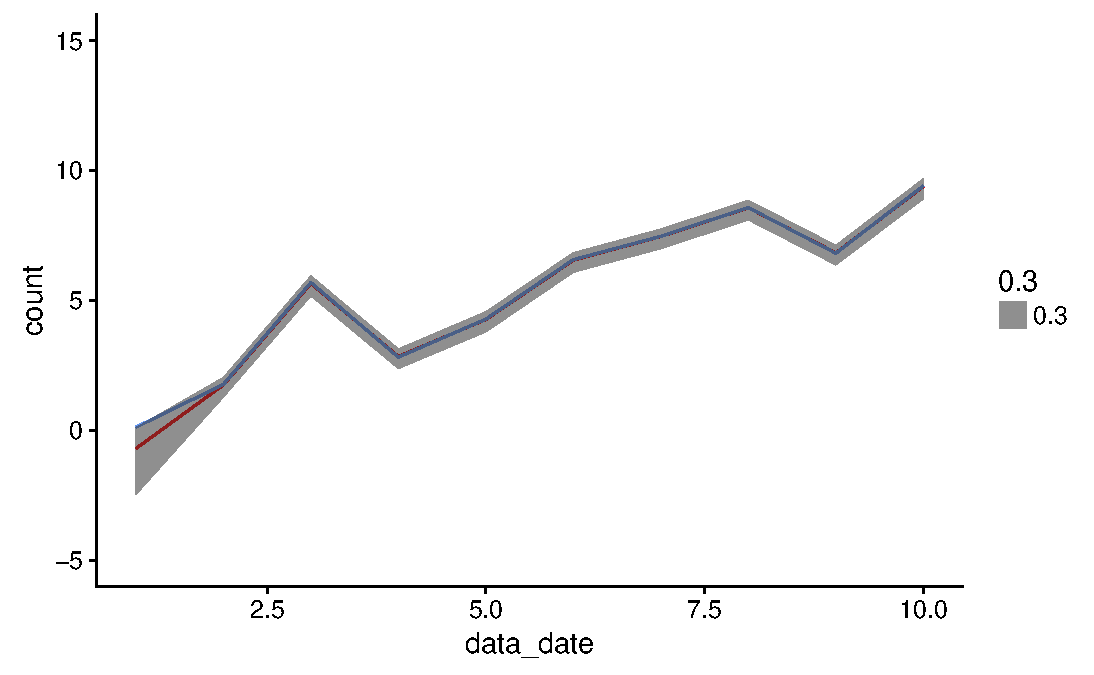
\includegraphics[scale=.25]{/home/gcgibson/ssvgd/manuscript/ssvgd_locally_level.pdf}\label{fig:f1}}
  \hfill
  \subfloat[PF]{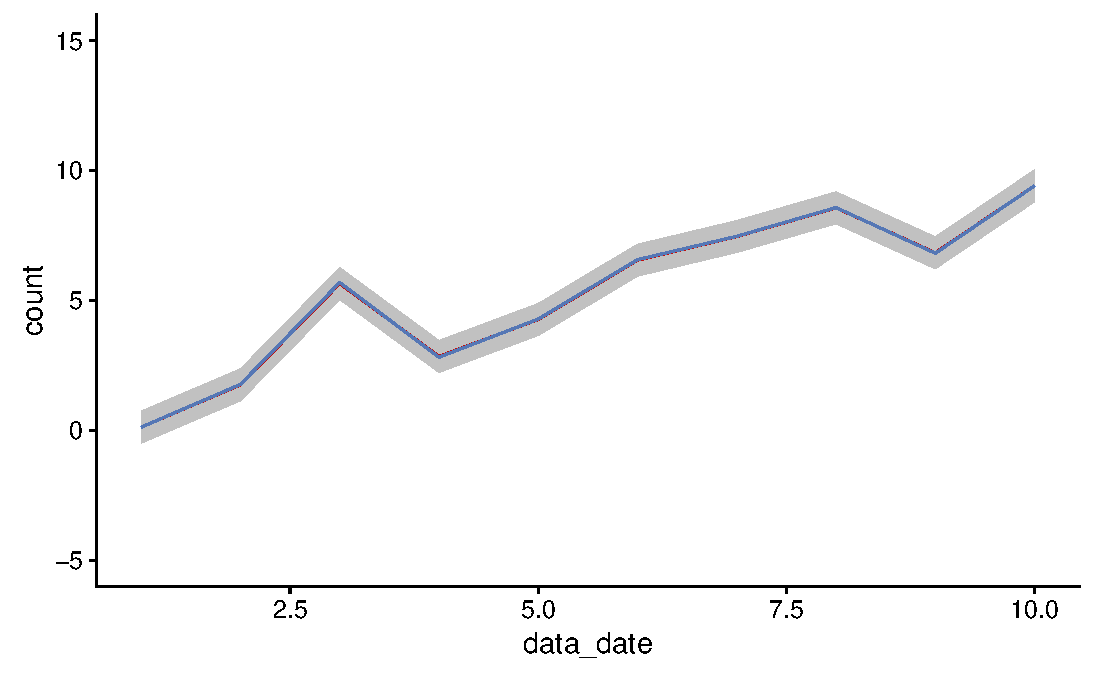
\includegraphics[scale=.25]{/home/gcgibson/ssvgd/manuscript/pf_locally_level.pdf}
\label{fig:f2}}
  \caption{Comparison of locally level Gaussian model}
\end{figure}



\subsection*{Poisson Observation Model With Seasonal State-Space Dynamics}

In order to evaluate the performance on more involved dynamics we consider the following state-space model.
$$\begin{pmatrix} X_{t,1} \\ X_{t,2} \end{pmatrix} = \begin{pmatrix} cos(2\pi/s) & sin(2\pi/s) \\ -sin(2\pi/s) & cos(2\pi/s) \end{pmatrix} \begin{pmatrix} X_{t-1,1} \\ X_{t-1,2} \end{pmatrix} $$
$$Y_t \sim Pois(e^{X_{t,1}})$$


\begin{figure}[!tbp]
\centering
\subfloat[SSVGD]{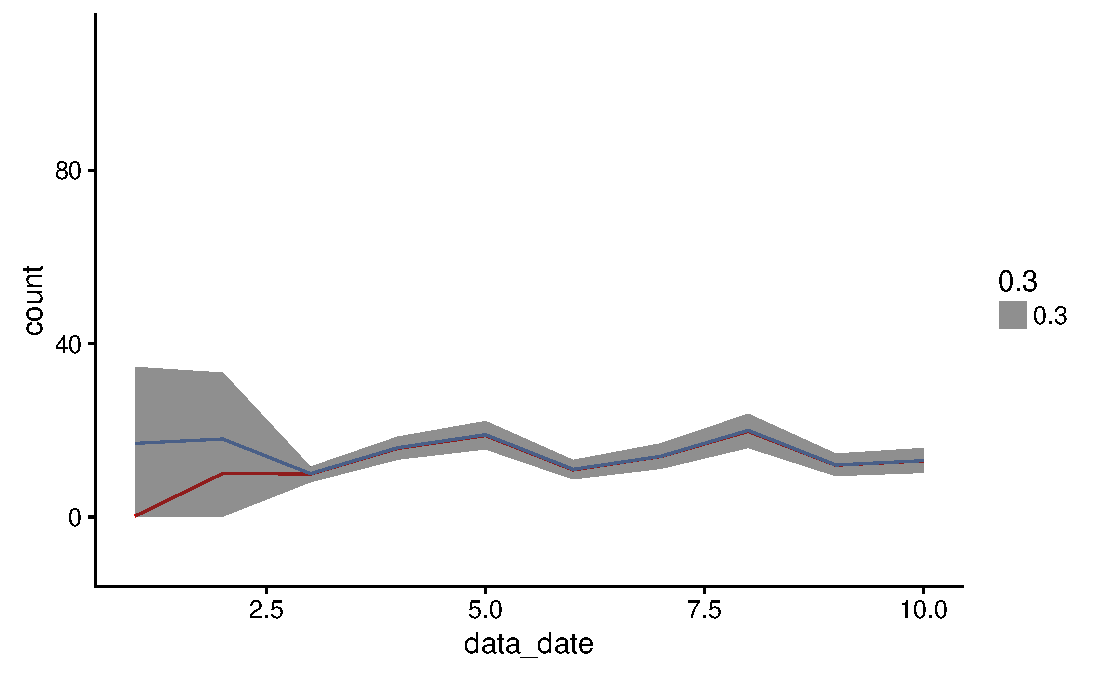
\includegraphics[scale=.25]{/home/gcgibson/ssvgd/manuscript/ssvgd_seasonal.pdf}\label{fig:f1}}
  \hfill
  \subfloat[PF]{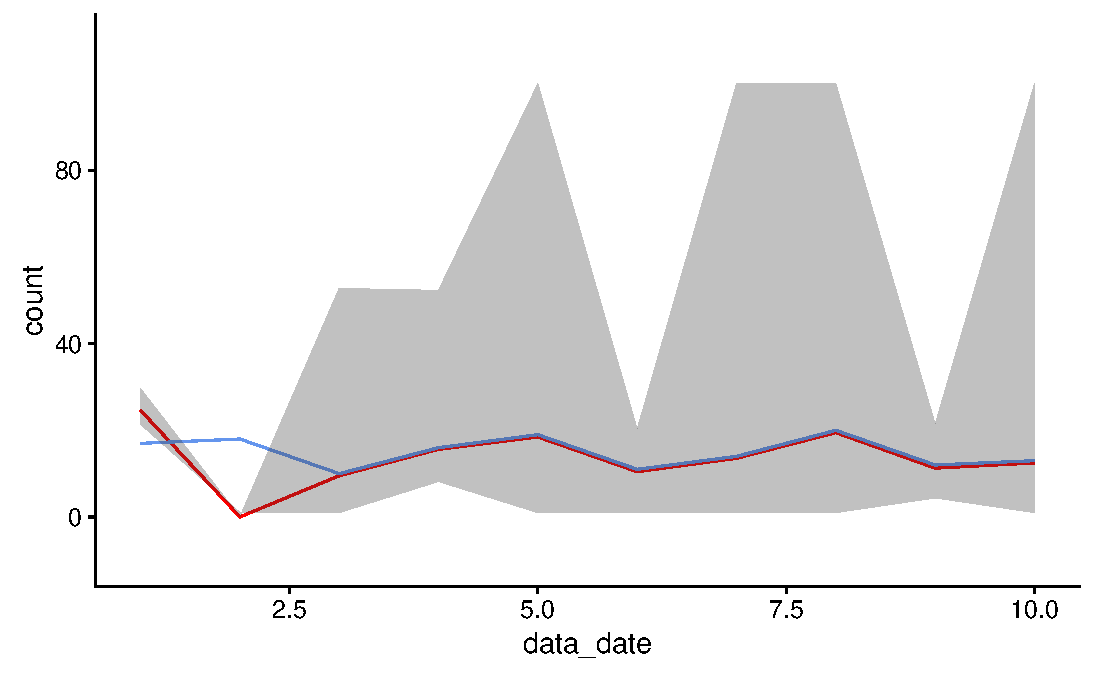
\includegraphics[scale=.25]{/home/gcgibson/ssvgd/manuscript/pf_seasonal.pdf}
\label{fig:f2}}
  \caption{Comparison of seasonal Poisson model}
\end{figure}

\subsection*{Divergent Particle Filter}

We next investigate the ability of SSVGD to perform in the presence of poor initialization. This is a well known issue with current particle filter implementations: starting far from a plausible value of $x_0$ forces all particles to receive weight $0$ under the likelihood, leading to a degenerate filtering distribution. However, under SSVGD, we can simply increase the number of iterations, allowing for arbitrarily poor starting points. Standard particle filtering algorithms use effective sample size as a measure of degeneracy. This is commonly defined as $$S^{pf}_{eff} = \frac{1}{\sum_i (w_t^i)^2}$$. The common rule of thumb is to not allow this quantity to drop below 50. The natural translation of this metric into particle filtering is compute the same metric based on the samples obtained by SSVGD. 


\subsection*{Results}
Standard particle filtering algorithms use effective sample size as a measure of degeneracy. This is commonly defined as $$S_{eff} = \frac{1}{\sum_i (w_i)^2}$$. The common rule of thumb is to not allow this quantity to fall below 50. Indeed, software implementations such as Biips throws an error if the number of effective particles falls below 50. We compute the effective sample size in an analogous way to the particle filter, where $w_i$ is defined as in the SIR particle filter. 

\subsection*{Discussion}

\cite{liu_stein_2016-4}


\printbibliography

\end{document}
